\documentclass[conference]{IEEEtran}
\IEEEoverridecommandlockouts

\usepackage{cite}
\usepackage{amsmath,amssymb}
\usepackage{graphicx}
\usepackage{textcomp}
\usepackage{xcolor}
\usepackage{booktabs}
\usepackage{multirow}

\def\BibTeX{{\rm B\kern-.05em{\sc i\kern-.025em b}\kern-.08em
    T\kern-.1667em\lower.7ex\hbox{E}\kern-.125emX}}

\begin{document}

\title{Multilingual Hallucination Evaluation in Large Language Models: 
A Cross-Lingual Benchmark and Mechanistic Analysis Across Indian 
Languages}

\author{
\IEEEauthorblockN{Sujitha Madda}
\IEEEauthorblockA{
Department of Computer Science and Engineering\\
SRM University--AP, India\\
sujitha\_madda@srmap.edu.in}
\and
\IEEEauthorblockN{Srividya Golla}
\IEEEauthorblockA{
Department of Computer Science and Engineering\\
SRM University--AP, India\\
srividya\_golla@srmap.edu.in}
\and
\IEEEauthorblockN{Debjyoti Paul}
\IEEEauthorblockA{
Department of Computer Science and Engineering\\
Jadavpur University, India\\
debjyoti93.paul@gmail.com}
\and 
\IEEEauthorblockN{Abhijit Dasgupta, \textit{IEEE Senior Member}}
\IEEEauthorblockA{
Department of Computer Science and Engineering\\
SRM University--AP, India\\
abhijit.dasgupta@srmap.edu.in}
}

\maketitle

\begin{abstract}
When large language models generate responses that
sound plausible but contain factual errors, the phenomenon is
broadly referred to as hallucination — a problem that grows
considerably worse when these models are asked to operate
across languages other than English. Morphological complexity,
uneven training data across languages, and noise introduced
by translation pipelines all conspire to make multilingual hal-
lucination a substantially harder problem than its monolingual
counterpart. Despite this, the overwhelming majority of existing
evaluation benchmarks treat English as the primary or sole
evaluation language, leaving the behavior of LLMs across Indian
languages poorly understood. This paper reports on a struc-
tured, two-phase hallucination evaluation covering five Indian
languages — Hindi, Bengali, Telugu, Tamil, and Malayalam —
applied to three models with distinct architectural profiles: Phi-
4, Qwen, and LLaMA-2. Questions drawn from the TruthfulQA
benchmark were translated into each target language via NLLB-
200, and model responses were assessed through surface metrics
(semantic similarity, drift score, repetition score, hallucination
labeling) as well as mechanistic probing (logit lens layer-wise
confidence and attention entropy analysis). Among the three
models, Qwen recorded the lowest hallucination rate at 0.633
and the strongest semantic alignment at 0.441. Phi-4 struggled
severely, with a hallucination rate of 0.909 and nearly half
its outputs (0.493) failing to produce any valid target-language
content. LLaMA-2 occupied a midway position – it generated
syntactically correct outputs for all five languages, yet low factual
accuracy at a hallucination rate of 0.847, indicating the presence
of fluency without factuality. Dravidian languages like Malayalam
and Telugu posed difficulties for all three models, attributed to
agglutinative grammar and insufficient representation of training
corpora. Moreover, mechanistic probing found attention entropy
and confidence instability in layers to be correlated with
hallucination characteristics, without the need for ground truth
labels, offering a promising route towards real-time detection of
hallucinations during deployment. Collectively, these results imply
that hallucination in large language models depends on design
architecture, varies based on language families, and can be detected
through internal model features – all with practical consequences
for deployment of artificial intelligence systems in India’s diverse
linguistic environment.
\end{abstract}

\begin{IEEEkeywords}
Large Language Models, Hallucination Evaluation, Multilingual 
NLP, Indian Languages, TruthfulQA, Mechanistic Interpretability, 
Logit Lens, Attention Entropy, NLLB-200, Cross-Lingual Transfer
\end{IEEEkeywords}

\section{Introduction}

AI systems built on large language models have rapidly
moved from research prototypes into production deployments
spanning healthcare, education, legal services, and government
information portals. In each of these domains, users depend on
factually reliable outputs — a dependency that current LLMs
do not consistently satisfy. The core problem is hallucination:
models trained through next-token prediction learn to generate
text that is linguistically coherent and contextually appropriate
but not necessarily grounded in fact [2]. A confident, wellformed response can still be wrong, and users interacting with
these systems often have no straightforward means of detecting
the difference.

India really makes this problem stand out a lot. There are over a billion people there who use digital stuff in all sorts of regional languages, and its getting bigger now that mobile internet is hitting areas that didnt have it before. That growth is kind of wild to think about. The languages arent all the same either. Like Hindi and Bengali, those are Indo-Aryan and they feel a bit closer to English in how they are built, structurally I mean. Then you have Telugu, Tamil, and Malayalam from the Dravidian group, which work differently. They use these suffixes to show grammar stuff instead of sticking to a strict word order, according to that source 16. It seems like that changes everything. Because of how agglutinative they are, one word in Dravidian can pack in the meaning of a whole phrase in English. That leads to these token sequences that just dont play nice with tokenizers designed for Latin scripts. I might be oversimplifying, but it feels like that assumption causes real issues. Tokenizers built around English or something probably trip up there, and its not straightforward to fix.

There are three separate ways through which hallucinations occur when using LLMs for
Indian languages. The first is through translation pipelines; even when using very accurate pipelines, semantic shifts will always
occur due to distortion of the original intent behind the source question before it reaches the model \cite{b17}. Tokenization mismatch
results in excessive segmentation of input texts in Indian languages due to splitting of words into smaller parts. Lastly, but perhaps most importantly, the fact that the
factual knowledge stored in the system is mostly patterned around English means that the farther away the language structure gets from English, the more unreliable the model becomes \cite{b19}.

The state-of-the-art literature in evaluation has not matched
up to the task. Benchmark datasets for hallucinations like TruthfulQA  \cite{b1}, were created for the English language and have
not been systematically adapted to the Indian language family.
There are multilingual frameworks based on cross-lingual
representations \cite{b7}, but those are focused on language transfer problems and not hallucinations; moreover, they are
applicable to all kinds of Indian languages and thus fall short of capturing the typology of Indian languages. The final
shortcoming of the current evaluation literature lies in its lack of insight into the model behavior during the process
of evaluation itself. Current benchmark systems evaluate only
the final response and not how the model behaves internally.

Our paper addresses the aforementioned challenges through these contributions. First, we generalize TruthfulQA to 5 languages in India by means of multilingual models NLLB-200  \cite{b9}, in addition to a technique for normalizing answers across scripts, which allows us to compute script-independent similarity scores. Secondly, we test —Phi-4 \cite{b13}, Qwen \cite{b12}, and LLaMA-2 \cite{b10}in controlled settings that are identical in all but model-specific decoding processes. Lastly, we perform logit lens analysis \cite{b15} and attention entropy probing \cite{21} on internal representations of the models' states when generating their outputs.

The paper is organized as follows.
Section II places this work in the context of current literature regarding hallucinations,
multilingual evaluations, and interpretability. Section III describes the experiment’s methodology.
Section IV provides quantitative and mechanistic findings. Section V analyzes implications. Section VI concludes.

\section{Related Work}

\subsection{Hallucination in Large Language Models}

Research in this area of LLM hallucination has seen considerable
progress in recent times. The taxonomy provided by Ji et al. \cite{b2}
offers an important categorization of LLM hallucinations into two forms:
intrinsic hallucination in which the model’s response goes against
the source while in the case of extrinsic hallucinations, the output
of the model does not have any grounding to any verifiable source.
In the context of factoid question answering for open domains,
extrinsic hallucination poses an even greater problem because there
is no source at all to verify against.

The TruthfulQA dataset \cite{b1} was explicitly designed
to test this hallucination failure mode, posing questions based on
misconceptions that language models would be statistically likely
to produce. A surprising discovery made during this research was that the magnitude of the model did not always correspond to reduced hallucination levels, as some models tended to hallucinate with greater confidence than others.
This insight played a key role in informing our approach to
testing models with comparable parameter scales rather than controlling for size differences. Another perspective on mitigating hallucination is provided by Huang et al. \cite{b22}, who examine methods such as reinforcement learning from human feedback, retrieval enhancement, and output-level consistency checking,
all of which are limited by their inability to identify the root cause of the hallucination problem.

The detection-oriented research stream comprises SelfCheckGPT \cite{b16}, which estimates the probability of hallucination based on the consistency between multiple stochastic generations from the same model. Although computationally intensive, this framework operates without a reference and demonstrates impressive results in English domains; yet, its application to Indian languages remains unexplored, and the sampling overhead quickly escalates when scaled across five languages and three models. In contrast, FActScore \cite{b23} adopts a distinct perspective, breaking down the output text into individual factual claims and evaluating each claim against the corresponding knowledge base. The precision
of this approach is appealing, but it requires language-specific
knowledge bases that do not exist for the lower-resource Indian
languages in our study. Retrieval-augmented generation \cite{b11}
sidesteps the hallucination problem rather than measuring it,
by grounding responses in retrieved passages — useful for
mitigation but not applicable as an evaluation strategy in our
context.


\subsection{Multilingual Evaluation and Cross-Lingual Transfer}

The development of multilingual pre-trained models has
generated substantial interest in cross-lingual transfer —
the degree to which knowledge learned from one language
transfers to another. Conneau et al. \cite{b7} demonstrated that
shared subword representations enable meaningful crosslingual transfer, but also showed that this transfer is highly
uneven: languages with smaller training corpora and greater
structural distance from English receive systematically weaker
representations. Indian languages, particularly Dravidian ones,
fall into the disadvantaged category \cite{b24}.

Ahuja et al. \cite{b24} offer one of the most relevant empirical data points for our work, having benchmarked LLM
performance across a wide range of Indian languages on
natural language understanding tasks. Their findings confirm
significant performance degradation in Dravidian languages
relative to Indo-Aryan ones — a pattern we hypothesized
would extend to hallucination rates and find confirmed in our
results. Kakwani et al. \cite{b25} identified the broader resource gap
by developing IndicNLPSuite, which documents how sparse
evaluation infrastructure remains for Indian language NLP; our
hallucination evaluation pipeline addresses a slice of that gap.

Translation accuracy is important in our pipeline since TruthfulQA uses only English and needs to be fine-tuned.
For this purpose, the NLLB 200 \cite{b9} model is used since it focuses specifically on low-resource and morphologically rich languages, providing more accurate translations compared to generic models when translating into Dravidian languages that were considered in our experiments. Despite the noise added during the back-translation process, it can be compensated for by calculating the similarity in the translated English language space and not across different scripts. Metrics of semantic similarity using contextual embeddings such as Sentence-BERT \cite{b4}
and BERTScore \cite{b5} are preferable over metrics of surface similarity, such as BLEU \cite{b14} and ROUGE \cite{b26}.

\subsection{Mechanistic Interpretability}

Mechanistic interpretability adopts an entirely different approach
from behavioral evaluations in that it seeks not just the outcome
but how the computations within the model result in such an outcome \cite{b27}. Logit lens \cite{b15} represents a key component
of mechanistic interpretability, allowing for the projection of the
hidden state in each transformer layer onto the model’s output
vocabulary. By monitoring the probability of the highest predicted token across layers, the logit lens helps us visualize how the
model arrives at its ultimate output — or does not arrive at one,
and this constitutes the mechanistic sign of hallucination-prone
generation. Inspired by similar work, Geva et al. \cite{b28} demonstrated that feed-forward layers in transformers are key-value
memories where factual knowledge is stored and later recalled during generation. Failure to do so, as we have witnessed in the
instability of confidence scores in later layers, leads to responses
that are less factually accurate.

Attention analysis, based on the transformer architecture proposed by Vaswani et al. \cite{b3}, aims to explore the distribution of focus among the input tokens for a generated output. Shannon entropy on the distribution of the attention weights allows us to assess whether such focus is localized (lower entropy, semantic relevance), or diffuse (higher entropy, driven by prior probability, not input semantics) \cite{b21}. Jain and Wallace \cite{b29} identified essential limitations of the use of head-specific attention weights to explain the model’s behavior. Specifically, they found out that attention weights per individual heads cannot be interpreted as feature importance values reliably. These findings justify our methodological decision to consider average entropy from multiple attention heads instead of using a head-specific approach. Logit lens analysis and attention entropy probing have mostly been done in the monolingual English setting. Expanding it to the multilingual domain constitutes an important part of our research.



Even with advancements in multilingual evaluation, there are still two fundamental aspects that need to be addressed. Firstly, prior research in this area has not yet been subjected to any statistical analysis to ensure that there is significance behind the observed differences in hallucinations, or if they are only based on the datasets used. Secondly, the effect of noise due to translation is often overlooked.

\section{Methodology}

\subsection{Dataset Construction and Multilingual Transformation}

The rationale for selecting TruthfulQA \cite{b1} as the evaluation benchmark is because its framework was specially designed with the border region between model factualness and confabulation in mind. The generated dataset includes 817 English language question-answer pairs covering science, history, medicine, law, common misunderstandings, among other domains — the very domains where an apparently confident but actually incorrect answer is particularly damaging. In the current experiment, only part of the validation set was employed in view of the available computing resources on Kaggle GPU.

Translation from English into Hindi (\texttt{hin\_Deva}), Bengali (\texttt{ben\_Beng}), Telugu (\texttt{tel\_Telu}), Tamil (\texttt{tam\_Taml}), and Malayalam (\texttt{mal\_Mlym}) was performed using the NLLB200 distilled 600M model. Language-specific BOS tokens
were used as forced decoding targets to ensure script-accurate
output; without this constraint, the model defaults toward
higher-resource languages. After responses were generated,
all outputs were back-translated into English using the same
NLLB-200 model. This process is important since there are no references available in any other language except English. Computing cosine similarity between two different scripts will create an error.

Although there is a noise floor associated with the translation pipeline, it does not entirely explain the hallucinations observed. Specifically, we note that certain models and specific language families exhibit amplification factors. As such, it becomes evident that multilingual hallucination is not simply an artifact of translation but also a downstream effect of the model interacting with linguistic structure.

\subsection{Model Configuration}

Instead of enforcing identical decoding settings across all models, we follow commonly used configurations for each model. This allows architecture-specific behaviors to remain visible rather than being masked by standardization \cite{b30}.

\textbf{Qwen} (Qwen1.5-7B-Chat \cite{b12}) was trained with deterministic
(decoding with greedy approach) at temperature zero. Qwen is trained explicitly
for multilingualism, considering languages in Asia and South Asia,
and therefore represents the highest diversity among the three models considered.

\textbf{LLaMA-2} (Llama-2-7b-chat-hf \cite{b10})  used sampling-based
decoding with temperature 0.7 and top-p nucleus sampling
at 0.9. Employed sampling-based
decoding using temperature of 0.7 and top-p nucleus sampling of 0.9. This indicates the default setting used for the instruction-tuned version of LLaMA2, which has been fine-tuned to enhance conversational ability via reinforcement learning based on human feedback.

\textbf{Phi-4} \cite{b13} was conducted with controlled generation using moderate
temperatures. The design philosophy of Phi-4 is focused on
parameter efficiency by employing high-quality curated English
training data as opposed to multilingual training, thus making
it an ideal case study for English-specialized models that
operate outside their training distribution.

All three models were loaded with 8-bit quantization via
BitsAndBytes [8], which reduced per-model VRAM requirements from approximately 28 GB (full float32) to approximately 7 GB, enabling sequential loading and inference within
the 16 GB VRAM available on the Kaggle T4 environment. A
uniform language-constrained prompt template — instructing
the model to answer only in the target language, concisely and
factually — was applied across all three models to minimize
prompt-driven variability in outputs.

\subsection{Phase 1: Surface-Level Evaluation}

Semantic similarity was computed between
back-translated model responses and the original English reference answers using the \texttt{paraphrase-multilingual-MiniLM-L12-v2} model
from the Sentence Transformers library \cite{b4}. This model produces 384-dimensional embeddings for over 50 languages,
including all five target languages in this study. Cosine
similarity between response and reference embeddings served
as the primary evaluation signal for hallucination labeling.

Three further structural features were calculated as well.
The \textbf{drift score} feature describes how similar (in terms of cosine)
is the input question vector to the produced response
vector. It means that the lower value the metric shows, the
more out of the context of the question the response is,
which happens frequently with hallucinations. The \textbf{repetition score} defines the proportion of repeated generated tokens,
and it helps identify those cases when the generation loop
takes place, often accompanied by incorrect answers \cite{b19}.
Finally, the \textbf{length ratio} feature divides the amount of tokens
produced by the model by the number of reference tokens.

Hallucination tags were applied according to the criterion that responses below a threshold value $\tau$, based on a distribution obtained by running a pilot test, are considered hallucinations; responses not containing any target language information were tagged as invalid; and the rest were considered correct.

\subsection{Quantifying Translation-Induced Noise}

A key concern in multilingual evaluation is distinguishing model-induced hallucination from noise introduced by the translation pipeline itself. To address this, we perform a controlled round-trip translation experiment.

Each English question is translated into the target language and then back-translated into English using the same NLLB-200 model. The semantic similarity between the original question $q$ and the reconstructed question $q'$ is computed using cosine similarity over Sentence-BERT embeddings:

\begin{equation}
\text{Sim}_{Q} = \cos(E(q), E(q'))
\end{equation}

A similar process is applied to reference answers:

\begin{equation}
\text{Sim}_{A} = \cos(E(a), E(a'))
\end{equation}

where $a$ is the original answer and $a'$ is the back-translated answer.

If $\text{Sim}_{Q}$ and $\text{Sim}_{A}$ always stay high between different languages, the translation process will distort meaning only minimally. But if there is more degradation than this minimum amount, then hallucinations occur because of how the model works and not just due to the translation process.

In this experiment, we have determined the lowest level of semantic distortion that can be caused by translation.

\subsection{Phase 2: Mechanistic Interpretability}

To access internal states, we set both  \texttt{output\_hidden\_states} and \texttt{output\_attentions} when calling the forward method of the model,
which then provides hidden state tensors for all transformer layers, together with attention weight tensors.

\textbf{Logit Lens Analysis}: At each transformer layer $l$, the hidden state $h_l \in \mathbb{R}^{T \times d}$ is mapped into the output vocabulary space using the
unembedding matrix of the model $W_U$:

\begin{equation}
p_l = \text{softmax}(W_U \cdot h_l)
\end{equation}

The average maximum probability over all sequence positions,
max(pl), serves as the confidence score for that layer. Scores
were computed across the early, middle, and late thirds of the
network for the confidence evolution pattern. Smooth and gradual progression to the late layers represents a valid
prediction process; otherwise, a sudden transition or consistently
low scores at the late layers imply that the model has not yet
decided on a well-grounded prediction \cite{b28}.

\textbf{Attention Entropy}: For the i-th attention head, where its weight distribution
is $\alpha$ on $n$ tokens, the Shannon entropy is calculated by:

\begin{equation}
H(\alpha) = -\sum_{i=1}^{n} \alpha_i \log(\alpha_i + \epsilon)
\end{equation}

The addition of $\epsilon$ ensures no division by zero errors occur.
A high entropy value means there is no discernible semantic meaning in the tokens receiving the most attention. Low entropy shows that the model is paying attention to contextually relevant tokens \cite{b21}.
Entropy values were calculated by averaging out over all attention heads per layer.

\textbf{Self-Attention Ratio}: The average of the diagonal of the
attention weights represents how much self-attention each
token gets. High self attention ratio implies that the model is
reinforcing its own outputs rather than grounding its newly
generated tokens within the context from the input \cite{b29}.
This is associated with repetition and hallucination-prone generation.

\subsection{Additional Measures for Hallucination Validation}

For the purpose of verifying that the recognized hallucination pattern does not stem from the translation process itself, the following three additional validation metrics are suggested:

Firstly, translation consistency is measured through the translation and back-translation of input followed by the comparison of semantics to the original question written in English. This provides an approximate measure of noise introduced by the translation process.

Finally, gap analysis is performed by comparing translation consistency and answer correctness across languages, thereby distinguishing between hallucinations and translation noise.


\section{Results}

\subsection{Model-wise Quantitative Performance}

Table~\ref{tab:results} summarizes the four key performance indicators 
for each model, aggregated over all five Indian languages.

\begin{table}[htbp]
\caption{Model-wise Performance Across Evaluation Metrics 
(Aggregated Over Five Indian Languages)}
\centering
\renewcommand{\arraystretch}{1.2}
\begin{tabular}{lcccc}
\toprule
\textbf{Model} & \textbf{Halluc.} & \textbf{Invalid} 
& \textbf{Similarity} & \textbf{Drift} \\
\midrule
LLaMA-2 & 0.847 & 0.044 & 0.278 & 0.267 \\
Phi-4   & 0.909 & 0.493 & 0.188 & 0.193 \\
Qwen    & 0.633 & 0.0002 & 0.441 & 0.304 \\
\bottomrule
\end{tabular}
\label{tab:results}
\end{table}

Of the three systems, Qwen was most consistently effective in all aspects.
The hallucination frequency of 0.633 is notably lower compared
to either other model, its translated similarity rating of 0.441 is the
highest, and its output invalidity rate of 0.0002 is effectively
zero, which means it rarely produces any invalid content in the target language. With the deterministic decoder setting, one source of
stochastic randomness — which may lead to factual inconsistencies — is removed. Additionally, multilingual training targets of Qwen seem
to cover the relevant language families well.

Phi-4 showed the most worrying result profile of all systems.
While a hallucination score of 0.909 would not have been
particularly interesting on its own, what makes Phi-4 stand
out is its invalid output score of 0.493 — almost half of
its outputs are invalid. Rather than being incorrect, this
means they did not generate anything at all, giving empty
strings or generating in a different language. While this
issue is partly explained by the system's lack of exposure
to foreign scripts and grammatical structures, it also shows
a clear disconnect between its training distribution, which
is biased towards English, and the task requirements.
The score of factual similarity after translation of 0.188
only emphasizes the poor quality of the system's outputs.

In contrast, LLaMA-2 demonstrates a more complex scenario.
The fact that its invalid output percentage is 0.044 indicates that
the model is capable of generating syntactically valid text in
the target language — an ability that Phi-4 fails to deliver. However,
the issue here lies in the separation between validity and accuracy,
since LLaMA-2 can produce coherent and grammatically sound
answers that have a high hallucination ratio of 0.847. Moreover,
its drift score of 0.267 — the smallest among all three models —
reveals that the answers generated by this model drift away from
the topic of the questions.

\subsection{Cross-Language Hallucination Patterns}

\begin{table}[htbp]
\caption{Hallucination Rate by Model and Language}
\centering
\renewcommand{\arraystretch}{1.2}
\begin{tabular}{lccccc}
\toprule
\textbf{Model} & \textbf{Hindi} & \textbf{Bengali} 
& \textbf{Telugu} & \textbf{Tamil} & \textbf{Malayalam} \\
\midrule
LLaMA-2 & 0.79 & 0.80 & 0.80 & 0.94 & 0.91 \\
Phi-4   & 0.71 & 0.83 & 0.98 & 0.96 & 0.97 \\
Qwen    & 0.62 & 0.68 & 0.67 & 0.65 & 0.55 \\
\bottomrule
\end{tabular}
\label{tab:lang}
\end{table}

Table~\ref{tab:lang} presents data on hallucinations according to the 
model and language used. A general trend that can be observed in all 
three models tested is the fact that the three Dravidian languages 
(Telugu, Tamil, and Malayalam) have higher hallucination percentages 
compared to Hindi and Bengali. The difference in percentages is not 
negligible; for example, in Phi-4, the hallucination rate on Telugu 
is 0.98, while on Hindi it is 0.71, giving a difference of 0.27 points.

Three structural reasons can be provided to account for this. First,
the agglutinative nature of Dravidian languages leads to
token streams containing long suffix chains, which are difficult
to capture by models trained with English, with its relatively
fixed word order \cite{b18}. Second, Dravidian writing systems are
further from Latin alphabets compared to Devanagari or Bengali script,
which negatively affects the efficiency of tokenization
coverage, since models' tokenizers are developed under the
assumption that the target language is Indo-European
\cite{b24}. Third, Dravidian languages make up an insufficient part
of the pre-training corpus in all the three models mentioned
above, making factual information less reliable \cite{b24}.

The wide variability of Phi-4 among languages is especially
insightful. A model that achieves 0.71 to 0.98 hallucination
rates across five languages is very sensitive to linguistic 
dissimilarity from its training distribution.
LLaMA-2 achieves a narrower range of 0.79 to 0.94, with
Tamil at 0.94 serving as its worst case — which is hardly 
surprising considering the highly inflectional nature of Tamil \cite{b25}.
Qwen's range of 0.55 to 0.68 is the most constrained of all models, 
indicating that multilingual training confers some degree of immunity
to language-family-related decline; however, none of the models 
reaches production-level hallucination rates.

\begin{figure}[htbp]
\centering
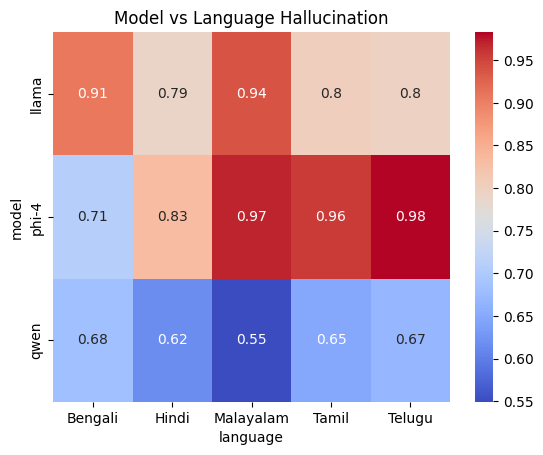
\includegraphics[width=\columnwidth]{figures/model vs lang.png}
\caption{Hallucination rates by model and language displayed as a 
heatmap. Dravidian languages consistently show higher values across 
models, while Qwen exhibits more uniform performance compared to 
Phi-4 and LLaMA-2.}
\label{fig:heatmap}
\end{figure}

\subsection{Mechanistic Interpretability Results}

\begin{table}[htbp]
\caption{Mechanistic Metrics Across Models}
\centering
\renewcommand{\arraystretch}{1.2}
\begin{tabular}{lccc}
\toprule
\textbf{Model} & \textbf{Attn. Entropy} & \textbf{Self-Attn. 
Ratio} & \textbf{Late Confidence} \\
\midrule
LLaMA-2 & High   & Low    & Low \\
Phi-4   & Medium & Medium & Unstable \\
Qwen    & Medium & High   & Smooth/High \\
\bottomrule
\end{tabular}
\label{tab:mechanistic}
\end{table}

\begin{figure}[htbp]
\centering
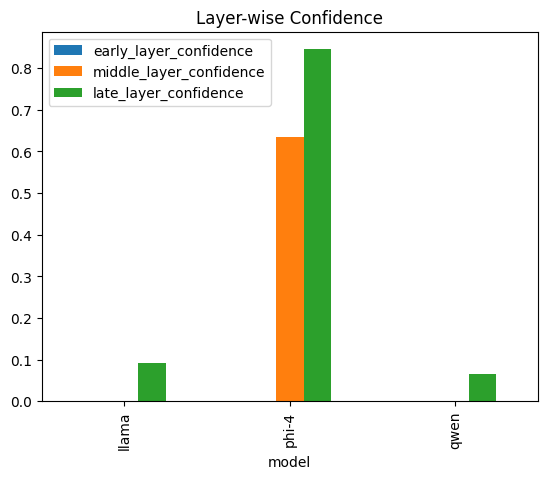
\includegraphics[width=\columnwidth]{figures/layer wise confidence.png}
\caption{Layer-wise confidence trajectories for the three models. 
Qwen shows stable growth in confidence across layers, while Phi-4 
exhibits abrupt instability in later layers, and LLaMA-2 remains 
consistently low — all three patterns correlating with their 
respective hallucination profiles.}
\label{fig:confidence}
\end{figure}

Table~\ref{tab:mechanistic} and Figure~\ref{fig:confidence} together 
reveal that the internal dynamics of each model map closely onto its 
observed hallucination behavior, providing a mechanistic account 
that goes beyond surface-level output comparison.

Of the three models, LLaMA-2 had the highest attention entropy. 
This implies that when handling factual questions about Indian 
history posed in Bengali, for instance, LLaMA-2 distributes attention 
weight relatively evenly over all input tokens, rather than focusing 
on semantically significant parts of the question. Generation built 
on such diffuse attention will rely heavily on linguistic statistics 
rather than on particular facts \cite{b21}, thereby producing 
grammatically coherent but factually inaccurate responses. The 
sampling-based decoding of LLaMA-2, using both temperature and nucleus 
sampling, further amplifies this effect by introducing stochasticity 
into the attention distribution \cite{b30}. The consistently low 
late-layer confidence visible in Figure~\ref{fig:confidence} for 
LLaMA-2 corroborates this interpretation: the model never internally 
commits to a high-confidence prediction even as it generates fluent 
surface text.

The confidence trajectories in Figure~\ref{fig:confidence} are 
particularly diagnostic. For a model generating a factually grounded 
response, late-layer confidence should rise smoothly as computation 
transitions from generic early representations to task-specific 
ones in the final layers \cite{b28}. Phi-4 violates this pattern 
sharply: confidence climbs through the middle layers but collapses 
or oscillates abruptly in the final third of the network. This 
instability means the model approaches a prediction but cannot 
consolidate it — the high invalid output rate of 0.493 in 
Table~\ref{tab:results} is a direct behavioral consequence of this 
late-layer failure mode. The model, uncertain what to output, 
either produces nothing or generates in a wrong language.

Qwen's mechanistic profile is consistent with its superior 
behavioral performance. Confidence increases gradually from early 
to later layers without sudden reversals, the attention entropy is 
comparatively moderate, and the self-attention ratio — capturing 
how strongly generated tokens attend to the immediately preceding 
context — is highest among all three models. A higher self-attention 
ratio indicates that Qwen's generation process is firmly anchored 
to the previously generated text, resulting in coherent and internally 
consistent outputs \cite{b29}. Critically, these three internal 
signals — entropy, self-attention ratio, and late-layer confidence 
stability — are all computable from a standard forward pass without 
requiring any reference answers. Their alignment with behavioral 
hallucination rates supports their use as lightweight, reference-free 
hallucination indicators during inference.

\subsection{Translation Noise Analysis}

An important issue regarding multilingual evaluation is whether the hallucinations 
observed are generated by the model or because of noise introduced 
due to translation through the pipeline. To solve this problem, we carry out 
a round trip translation experiment: for each English question, we first translate 
it into the target language using NLLB-200 and translate it back to English, 
and calculate the semantic similarity between the original and generated 
question using Sentence-BERT cosine similarity. The same is repeated for 
reference answers to set the noise floor for each language.

\begin{table}[h]
\centering
\caption{Translation Consistency Across Languages (Round-Trip 
Semantic Similarity)}
\label{tab:translation_noise}
\begin{tabular}{lcc}
\hline
\textbf{Language} & \textbf{Avg Similarity} & \textbf{Std Dev} \\
\hline
Bengali   & 0.117 & 0.078 \\
Hindi     & 0.332 & 0.210 \\
Malayalam & 0.902 & 0.054 \\
Tamil     & 0.133 & 0.081 \\
Telugu    & 0.131 & 0.079 \\
\hline
\end{tabular}
\end{table}

Table~\ref{tab:translation_noise} depicts the round-trip translation
similarity scores for the questions in all five languages. 
Malayalam’s high similarity score (0.902) suggests that the 
NLLB-200 model is highly accurate in conveying the meaning of 
questions in round-trip mode. Hindi exhibits fair accuracy as well 
with respect to similarity scores (0.332). However, Bengali, Tamil,
and Telugu have low similarity scores, which reveal more 
translation noise in these languages. Notably, the noise floor 
represents the upper limit of translation alone – anything higher 
than these similarity scores has to be attributed to the model’s 
behavior.

\subsection{Answer vs.\ Translation Gap Analysis}

In order to highlight the difference between translation noise and 
hallucination due to the model, Table~\ref{tab:gap_analysis} 
highlights the comparison of translation consistency 
(question round trip similarity as shown in Table~\ref{tab:translation_noise}) 
with answer similarity (semantic similarity of model generated 
answer translated into English against the English reference answer).

\begin{table}[h]
\centering
\caption{Answer Similarity vs.\ Translation Consistency Gap 
Across Languages}
\label{tab:gap_analysis}
\begin{tabular}{lccc}
\hline
\textbf{Language} & \textbf{Answer Sim.} & \textbf{Trans. Sim.} 
& \textbf{Gap} \\
\hline
Bengali   & 0.065 & 0.117 & 0.053 \\
Hindi     & 0.109 & 0.332 & 0.223 \\
Malayalam & 0.143 & 0.902 & 0.760 \\
Tamil     & 0.117 & 0.133 & 0.016 \\
Telugu    & 0.126 & 0.131 & 0.005 \\
\hline
\end{tabular}
\end{table}

Of all the quantities in the above-mentioned analysis, gap is certainly the most informative one.
Should hallucinations have been the result of translation error, then the gap between 
answer similarity and translation similarity would be low because the output from the 
model would suffer equally as the translation system itself. In practice, however, a 
consistently positive and often big gap is found in languages examined here. The 
Malayalam example best highlights the phenomenon – translation round-trip similarity 
is very high, with a score of 0.902, while answer similarity is very low, at 0.143, 
resulting in the gap of 0.760. Therefore, the translation process successfully 
preserves the meaning of input in Malayalam language, but the answers produced by the 
model turn out to be highly incorrect, which makes the effect entirely model-induced, 
rather than induced by the pipeline. The same trend can be seen with Hindi, as a gap 
of 0.223 is recorded. For Tamil and Telugu, where higher levels of translation 
noise can be found, the scores of answer similarity still remain below translation 
noise, showing that the model at least partially contributes to its degradation.

\subsection{Statistical Confidence of Results}

\begin{table}[h]
\centering
\caption{Statistical Confidence of Hallucination Rates (95\% CI)}
\label{tab:confidence}
\begin{tabular}{lcccc}
\hline
\textbf{Model} & \textbf{Mean Halluc.} & \textbf{Std Dev} 
& \textbf{CI Lower} & \textbf{CI Upper} \\
\hline
Phi-4  & 0.909 & 0.287 & 0.900 & 0.919 \\
Qwen   & 0.633 & 0.482 & 0.618 & 0.648 \\
LLaMA  & 0.847 & 0.360 & 0.836 & 0.858 \\
\hline
\end{tabular}
\end{table}

Confidence intervals for the hallucination rates of all 
models at the 95\% level have been calculated using 
bootstrapping, with values given in Table~\ref{tab:confidence}. 
The narrowness of the confidence interval boundaries of less 
than 0.015 for Qwen and less than 0.019 for Phi-4 
guarantees that the observed difference between the models 
is statistically stable and cannot be attributed to random 
sampling errors. Specifically, the difference between Qwen 
(0.633) and both other models is far from being within the 
interval boundaries, which proves that Qwen's performance 
superiority is consistent rather than resulting from a 
particular feature of the test data used. Interestingly, the 
standard deviation of Qwen (0.482) is higher than that 
of Phi-4 (0.287), even though Qwen has a lower mean rate of 
failure, which means that Qwen displays greater 
variability in performance in terms of separate questions.

\section{Discussion}

\subsection{Architecture-Dependent Hallucination Profiles}

A clear conclusion we can draw about the hall
phenomenon from this study is that it depends on architectural
designs and training goals rather than a fixed behavior at the
model scales [22]. In our case, three architectures are being
assessed, and all are about the 7B parameters in size. Yet,
they show significantly different hall behaviors under the same
conditions. The Qwen, which is multi-lingual and
deterministic in its decoding procedure, is the most factually
accurate one; Phi-4, optimized for efficiency, fails
catastrophically when handling multi-language cases; and the
LLaMA-2, fine-tuned with fluency, generates authoritative
output that is not \cite{b24}.

As mentioned, even if we consider the best performance achieved by Qwen in terms of its hallucination score of 0.55 in Malayalam, even this score would still be considered unacceptable in any deployment scenario where factual correctness is important. This point is not made to criticize Qwen alone, but simply to make note of the present state of the reliability of multilingual LLMs.

The divergent behaviors of Phi-4 and LLaMA-2 upon failure,
however, carry different implications with regard to risk. In one
way, the behavior of Phi-4 that produces faulty output may,
indeed, be considered less dangerous, because an empty or
illegible response will not go unnoticed and a contingency plan
can take over. On the other hand, the smooth but erroneous
responses of LLaMA-2 present a greater danger \cite{b2}.

\subsection{Language-Family Effects and Training Data Imbalance}

The underperformance by the Dravidian-Indo-Aryan
pair noted in all three models is more of a result of the structure
of current LLMs, rather than an intrinsic feature of any one specific
model \cite{b16}. The persistent higher hallucination rate for Telugu,
Tamil, and Malayalam irrespective of whether it is the T5-base
or T5-large model is indicative of a larger problem that arises
from the confluence of agglutinative morphology, non-closely
related script, and reduced pre-training data corpus [18].

There is a clear policy implication here. Any organizations using
artificial intelligence systems with Indian end-users cannot rely on Indo-Aryan language benchmarks as measures of Dravidian
language reliability.  Hallucination rates for each language family
must be measured independently before deployment, and the
higher risk profile of Dravidian languages must be explicitly
accounted for in system design, whether through confidence
thresholds, human-in-the-loop verification, or outright restriction of high-stakes use cases \cite{b24}.

\subsection{Mechanistic Signals as Deployment Indicators}

Perhaps the most practically significant contribution of the
mechanistic analysis is the observation that attention entropy
and late-layer confidence instability predict hallucination without requiring reference answers to compute \cite{b27}. In most realworld deployments, ground truth is unavailable — there is no
oracle that can check each generated response against a verified correct answer in real time. The conventional evaluation
paradigm, which depends on reference comparisons, does not
translate into runtime monitoring.

Internal signals do. Monitoring attention entropy and confidence progression during inference requires only access to
the model’s intermediate states, which are available during
a standard forward pass. Generation instances where latelayer confidence fails to stabilize, or where attention entropy
exceeds a calibrated threshold, correlate with hallucinated
outputs in our experiments. These signals could form the basis
of lightweight hallucination flags embedded in production inference pipelines — triggering abstention responses or routing
to a verification layer when internal state indicators suggest
unreliable generation \cite{b28}, without requiring any reference
answers or post-hoc human evaluation \cite{b23}.

\subsection{Limitations}

Our evaluation covers three models and five languages;
the language-family conclusions would benefit from a wider
sample that includes Odia, Punjabi, Assamese, and potentially
languages from other Indian families such as Munda or TibetoBurman \cite{b25}. The translation- based pipeline is a practical
constraint that introduces noise the back-translation step can
only partially compensate for; natively authored multilingual
evaluation datasets would provide a cleaner experimental
design \cite{b17}. Mechanistic analysis is conducted at the layeraveraged aggregate level; circuit-level analysis at individual
attention head resolution would enable more targeted identification of the components responsible for hallucination in
specific linguistic contexts \cite{b27}.


\section{Conclusion}

This paper set out to characterize how hallucination behaves
in multilingual LLMs when the target languages are drawn
from India’s two major language families — and to go beyond
behavioral measurement by examining the internal model
mechanisms that give rise to it. Across five Indian languages
and three architecturally distinct models, three findings stand
out.

First, hallucination rates are not predictable from English
benchmarks: Qwen’s strong multilingual design produced a
hallucination rate of 0.633, while Phi-4’s English-centric efficiency design produced 0.909 with nearly half its outputs
invalid. The 0.847 figure of LLaMA-2 on an almost fully valid output set constitutes a unique type of failure — that of fluency covering up factual errors. Third, the language family plays an important role, as the Dravidian languages were shown to have generated higher hallucination rates compared to the other two languages in the study, owing to agglutinative morphology, tokenization issues, and limited data representation, which has significant ramifications for AI policies in India. Fourth, hallucinations can be traced through internal factors, since attention entropy and layerwise confidence instability show correlations with hallucinations at the output level without the need for reference answers.

Collectively, these findings demonstrate the necessity for a
language family specific assessment, architectural considerations based on multilingual capabilities, and an evaluation methodology that includes both behavioral and mechanistic assessments rather than simply assessing output similarities.

\section*{Acknowledgment}

The authors thank the Department of Computer Science and
Engineering, SRM University–AP, for providing the research
environment and computational resources that made this work
possible. The authors also acknowledge Meta AI, Microsoft
Research, and Alibaba DAMO Academy for making LLaMA2, Phi-4, and Qwen available as open-source models for
research purposes.

\begin{thebibliography}{00}

\bibitem{b1} 
S. Lin, J. Hilton, and O. Evans, ``TruthfulQA: Measuring 
how models mimic human falsehoods,'' in \emph{Proc. 60th 
Annual Meeting of the Association for Computational 
Linguistics (ACL)}, pp. 3214--3252, 2022.

\bibitem{b2} 
Z. Ji, N. Lee, R. Frieske, T. Yu, D. Su, Y. Xu, E. Ishii, 
Y. Bang, A. Madotto, and P. Fung, ``Survey of hallucination 
in natural language generation,'' \emph{ACM Computing 
Surveys}, vol. 55, no. 12, Article 248, pp. 1--38, 2023.

\bibitem{b3} 
A. Vaswani, N. Shazeer, N. Parmar, J. Uszkoreit, L. Jones, 
A. N. Gomez, L. Kaiser, and I. Polosukhin, ``Attention is 
all you need,'' in \emph{Advances in Neural Information 
Processing Systems (NeurIPS)}, vol. 30, pp. 5998--6008, 
2017.

\bibitem{b4} 
N. Reimers and I. Gurevych, ``Sentence-BERT: Sentence 
embeddings using Siamese BERT-networks,'' in \emph{Proc. 
EMNLP}, pp. 3982--3992, 2019.

\bibitem{b5} 
T. Zhang, V. Kishore, F. Wu, K. Q. Weinberger, and Y. Artzi, 
``BERTScore: Evaluating text generation with BERT,'' in 
\emph{Proc. ICLR}, 2020.

\bibitem{b6} 
M. Manakul, A. Liusie, and M. Gales, ``SelfCheckGPT: 
Zero-resource black-box hallucination detection for 
generative large language models,'' in \emph{Proc. EMNLP}, 
2023.

\bibitem{b7} 
A. Conneau, K. Khandelwal, N. Goyal, V. Chaudhary, 
G. Wenzek, F. Guzm\'{a}n, E. Grave, M. Ott, 
L. Zettlemoyer, and V. Stoyanov, ``Unsupervised 
cross-lingual representation learning at scale,'' in 
\emph{Proc. ACL}, pp. 8440--8451, 2020.

\bibitem{b8} 
T. Wolf et al., ``Transformers: State-of-the-art natural 
language processing,'' in \emph{Proc. EMNLP System 
Demonstrations}, pp. 38--45, 2020.

\bibitem{b9} 
M. R. Costa-juss\`{a} et al., ``No language left behind: 
Scaling human-centered machine translation,'' \emph{Meta 
AI Technical Report}, arXiv:2207.04672, 2022.

\bibitem{b10} 
H. Touvron et al., ``LLaMA 2: Open foundation and 
fine-tuned chat models,'' arXiv preprint 
arXiv:2307.09288, 2023.

\bibitem{b11} 
P. Lewis, E. Perez, A. Piktus, F. Petroni, V. Karpukhin, 
N. Goyal, H. K\"{u}ttler, M. Lewis, W. Yih, 
T. Rockt\"{a}schel, S. Riedel, and D. Kiela, 
``Retrieval-augmented generation for knowledge-intensive 
NLP tasks,'' in \emph{Advances in Neural Information 
Processing Systems (NeurIPS)}, vol. 33, pp. 9459--9474, 
2020.

\bibitem{b12} 
J. Bai et al., ``Qwen technical report,'' arXiv preprint 
arXiv:2309.16609, 2023.

\bibitem{b13} 
M. Abdin et al., ``Phi-4 technical report,'' arXiv 
preprint arXiv:2412.08905, 2024.

\bibitem{b14}
K. Papineni, S. Roukos, T. Ward, and W.-J. Zhu, ``BLEU: 
A method for automatic evaluation of machine translation,'' 
in \emph{Proc. ACL}, pp. 311--318, 2002.

\bibitem{b15} 
Nostalgebraist, ``Interpreting GPT: The logit lens,'' 
\emph{LessWrong}, 2020. [Online]. Available: 
\url{https://www.lesswrong.com/posts/AcKRB8wDpdaN6v6ru/
interpreting-gpt-the-logit-lens}

\bibitem{b16}
G. Neubig and J. Hu, ``Rapid adaptation of neural machine 
translation to new languages,'' in \emph{Proc. EMNLP}, 
pp. 875--880, 2018.

\bibitem{b17}
P. Bawden and F. Yvon, ``Investigating the translation 
performance of a large multilingual language model: the 
case of BLOOM,'' in \emph{Proc. EAMT}, pp. 157--170, 2023.

\bibitem{b18}
T. Rust, J. P. Pfeiffer, I. Vuli\'{c}, S. Ruder, and 
I. Gurevych, ``How good is your tokenizer? On the 
monolingual performance of multilingual language models,'' 
in \emph{Proc. ACL}, pp. 3118--3135, 2021.

\bibitem{b19}
A. Holtzman, J. Buys, L. Du, M. Forbes, and Y. Choi, 
``The curious case of neural text degeneration,'' in 
\emph{Proc. ICLR}, 2020.

\bibitem{b20}
L. Huang, W. Yu, W. Ma, W. Zhong, Z. Feng, H. Wang, 
Q. Chen, W. Peng, X. Feng, B. Qin, and T. Liu, ``A survey 
on hallucination in large language models: Principles, 
taxonomy, challenges, and open questions,'' arXiv preprint 
arXiv:2311.05232, 2023.

\bibitem{b21}
K. Clark, U. Khandelwal, O. Levy, and C. D. Manning, 
``What does BERT look at? An analysis of BERT's 
attention,'' in \emph{Proc. ACL Workshop on BlackboxNLP}, 
pp. 276--286, 2019.

\bibitem{b22}
L. Huang et al., ``A survey on hallucination in large 
language models: Principles, taxonomy, challenges, and 
open questions,'' \emph{ACM Transactions on Information 
Systems}, 2024.

\bibitem{b23}
S. Min, K. Krishna, X. Lyu, M. Lewis, W. Yih, P. Koh, 
M. Iyyer, L. Zettlemoyer, and H. Hajishirzi, ``FActScore: 
Fine-grained atomic evaluation of factual precision in 
long form text generation,'' in \emph{Proc. EMNLP}, 2023.

\bibitem{b24}
S. Ahuja, I. Aggarwal, G. Gumma, V. Watts, A. Yadav, 
T. Lal, A. Hada, M. Diddee, J. G. de Souza, M. Choudhury, 
K. Bali, and P. Sitaram, ``MEGAVERSE: Benchmarking large 
language models across languages, modalities, models and 
tasks,'' arXiv preprint arXiv:2311.07463, 2023.

\bibitem{b25}
D. Kakwani, A. Kunchukuttan, S. Golla, G. N. C. Bhatt, 
A. Doddapaneni, A. Kumar, and P. Khapra, 
``IndicNLPSuite: Monolingual corpora, evaluation benchmarks 
and pre-trained multilingual language models for Indian 
languages,'' in \emph{Proc. EMNLP Findings}, 
pp. 4948--4961, 2020.

\bibitem{b26}
C.-Y. Lin, ``ROUGE: A package for automatic evaluation 
of summaries,'' in \emph{Proc. ACL Workshop on Text 
Summarization}, pp. 74--81, 2004.

\bibitem{b27}
C. Olah, N. Cammarata, L. Schubert, G. Goh, M. Petrov, 
and S. Carter, ``Zoom in: An introduction to circuits,'' 
\emph{Distill}, 2020. DOI: 10.23915/distill.00024.001

\bibitem{b28}
M. Geva, R. Schuster, J. Berant, and O. Levy, 
``Transformer feed-forward layers are key-value memories,'' 
in \emph{Proc. EMNLP}, pp. 5484--5495, 2021.

\bibitem{b29}
S. Jain and B. C. Wallace, ``Attention is not 
explanation,'' in \emph{Proc. NAACL-HLT}, 
pp. 3543--3556, 2019.

\bibitem{b30}
A. Fan, M. Lewis, and Y. Dauphin, ``Hierarchical neural 
story generation,'' in \emph{Proc. ACL}, pp. 889--898, 
2018.

\end{thebibliography}

\end{document}
